\chapter{Space Case}
\section{Introduction}
  
In addition to vowel duration, I also include vowel dispersion measured by the euclidean distance from the center of each singer's vowel space on the (f1, f2) plane. A larger vowel perimeter generally corresponds to hyper-articulation or clear speech, while a smaller perimeter with hypo-articulation or reduction \cite{lindblom1990, smiljanic2005}. In natural Estonian speech, reduction is only allowed on unstressed syllables, with /i/ being the most resistant \citep{eekMeister1998}. An early paper by Ross measured formant frequencies f1 and f2, finding a reduced vowel space in song compared to measurements in spoken Estonian\cite{ross1992}. However, upon examination of tokens included in the analysis, it is clear that the sample of sung syllable-notes consists entirely of syllables in non-initial positions of Estonian words: that is, the sample of vowels taken from  the song were all unstressed. Conversely, the spoken Estonian used for this comparison contained stressed and unstressed syllables. 


This measurement is included for two reasons: one, the acoustic correlates of prominence in both language and music are almost always not a single cue but a convergence of several cues. If duration is less available for word-level contrasts when it is constrained by musical meter, vowel dispersion is a viable candidate for indicating prominence in its stead.  The second reason is to follow up on the findings of \citep{ross1989,ross1992}, this time comparing vowel space in stressed and unstressed syllables within the song.  

\subsection{Previous Work}
An earlier study of vowel quality \cite{ross1992} found a reduction in the dispersion of vowels in regilaul singing compared to running speech. However, all vowel tokens in that study were taken from syllables that are unstressed at the words level, while the running speech comparison data included all stress positions. Thus we do not know if the vowel space is best predicted by {\it style} i.e., spoken or sung, or by word stress, or a combination of both. 
To begin probing this question further, I include measurements of vowel space of stressed and unstressed sung syllables. 
	\begin{itemize}
	\item \(HS\): stress/unstress contrasts will be evident in the nucleus in terms of hypo and hyper articulation. For this I measure both nucleus duration and vowel space dispersion. 
	\item \(HS_{\emptyset}\): vowel dispersion differences in syllables are random. 
	\end{itemize}

\subsection{Results}
A subset of the Q1 and Q2 vowels used for duration measurements above is taken,  containing only those five vowel phonemes which occur in both stressed and unstressed syllables at the word level: \(a, e, i, o, u\). The total number of vowels in this set is {\bf N}.
To account for physiological differences between singers, vowel dispersion is calculated as the euclidean distance of each token from the respective singer's vowel center in the (F1, F2) space. 


\begin{figure}[htb]
\centering
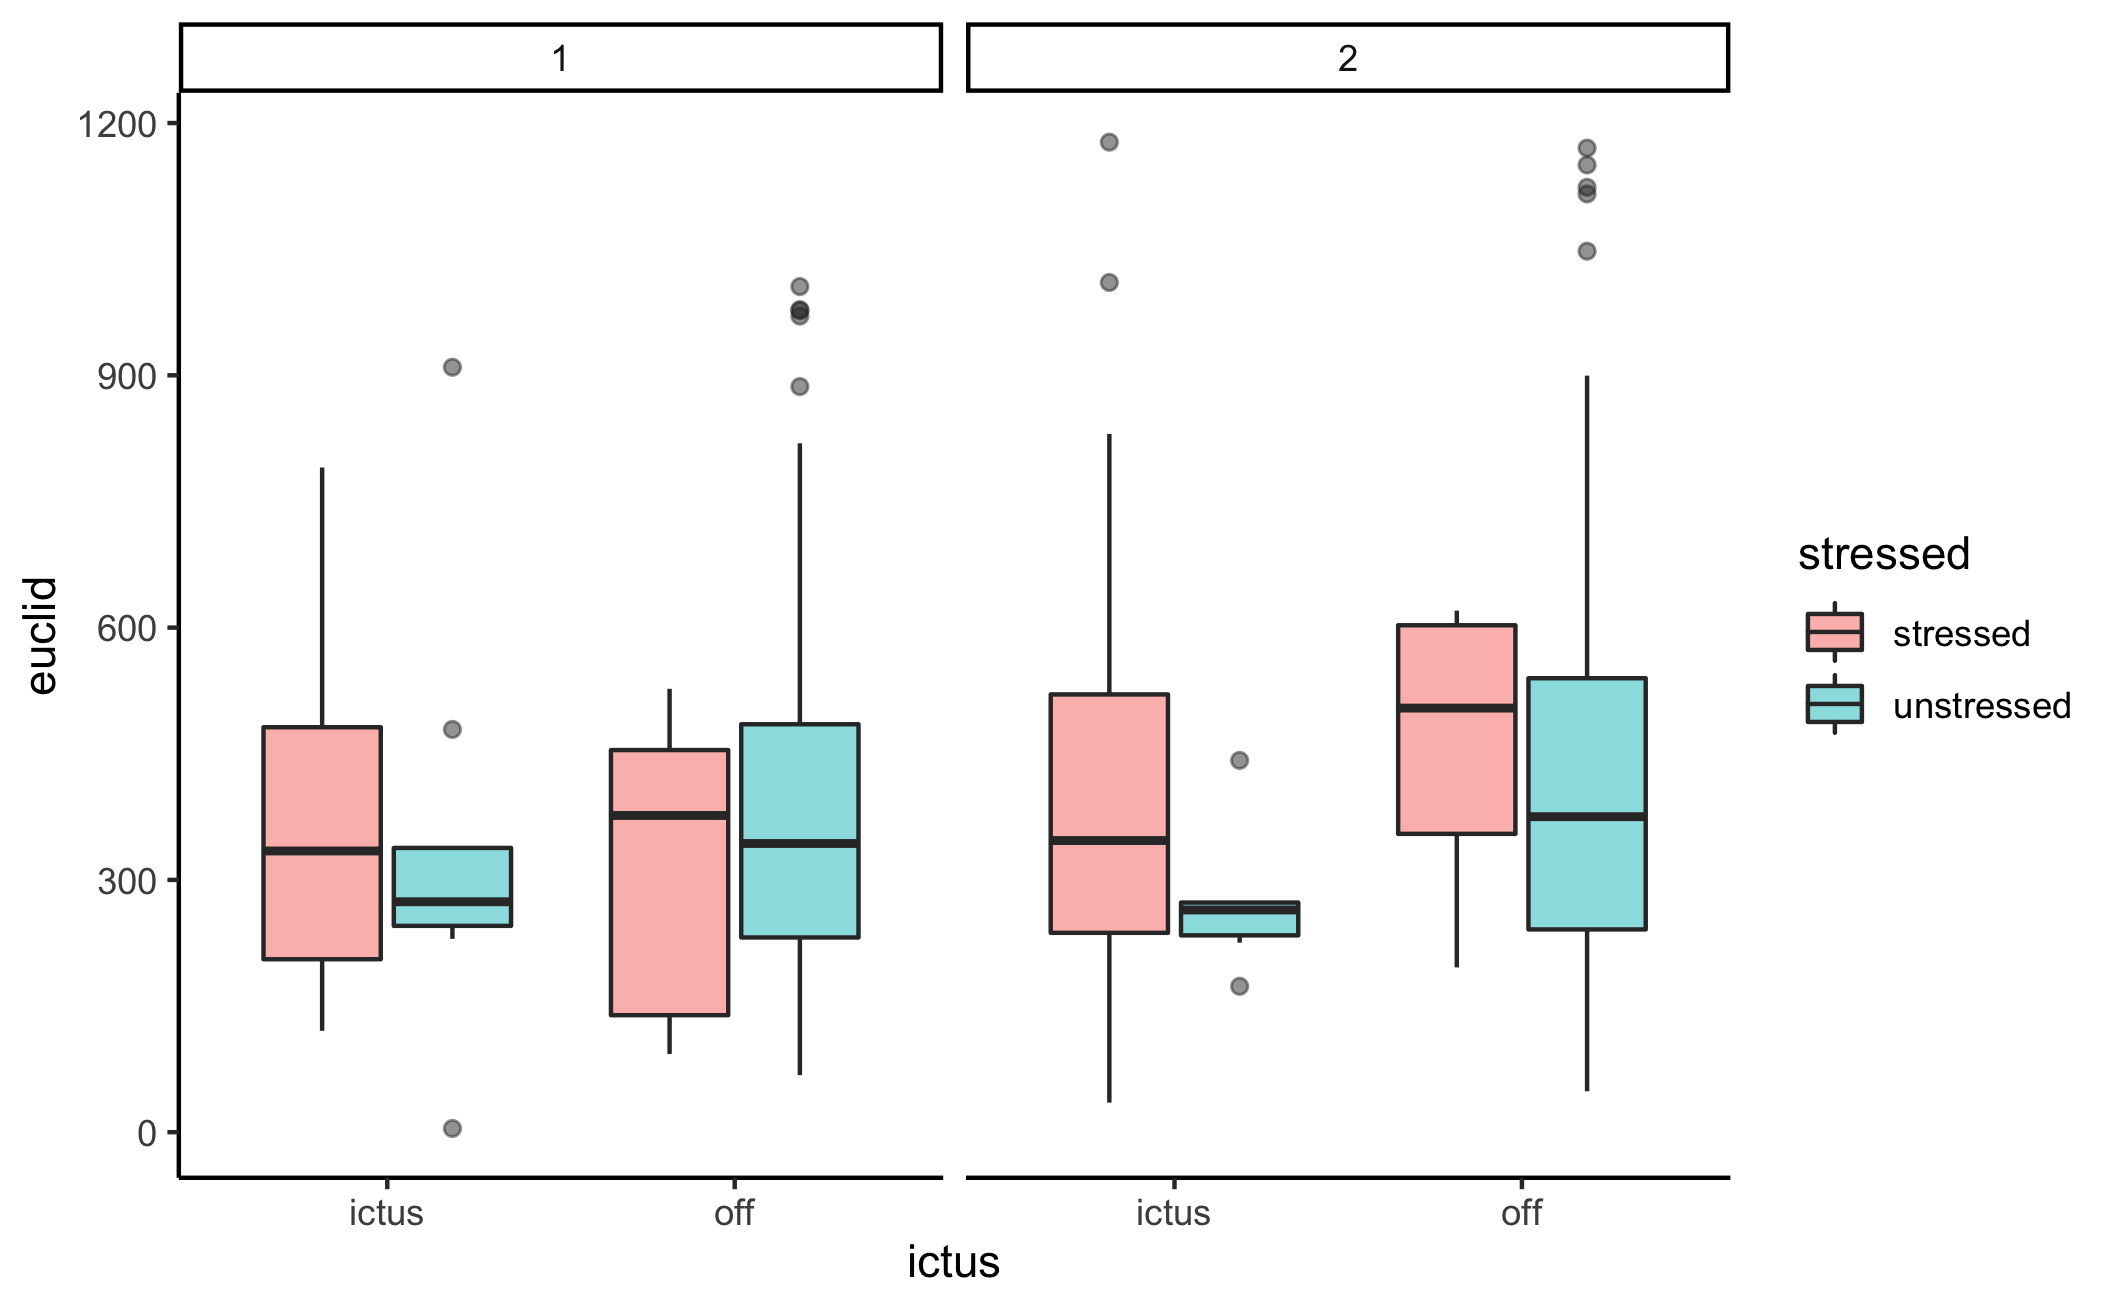
\includegraphics[width=\textwidth]{/Users/sarah/Git/regilaul_project/manuscript/results/space_strictus.png}
\caption{euclidean distance of vowels in stress and ictus}
\label{spcstrick}

\end{figure}
A pattern is marginally visible in the two graphs  \ref{spcstrick}, faceted by Q1 and Q2. Notice that in off-ictus position, vowel dispersion means of stressed syllables are higher than those of stressed syllables in ictus position. This indicates that stressed syllables falling off the beat are being compensated for their shortened vowels by way of increased articulation of quality. This pattern, however, doesn't shake out as statistically significant in the model. \\
A linear mixed effects model for vowel dispersion is constructed, but only the uninterpretable intercept shows significance. 
Comparison with null model is not statistically significant. Thus in the case of vowel dispersion, we fail to reject the null hypothesis. This could be due to the relatively smaller size of the data subset. 


